%%%%%%%%%%%%%%%%%%%%%%%%%%%%%%%%%%%%%%%%%
% Programming/Coding Assignment
% LaTeX Template
%
% This template has been downloaded from:
% http://www.latextemplates.com
%
% Original author:
% Ted Pavlic (http://www.tedpavlic.com)
%
% Note:
% The \lipsum[#] commands throughout this template generate dummy text
% to fill the template out. These commands should all be removed when 
% writing assignment content.
%
% This template uses a Perl script as an example snippet of code, most other
% languages are also usable. Configure them in the "CODE INCLUSION 
% CONFIGURATION" section.
%
%%%%%%%%%%%%%%%%%%%%%%%%%%%%%%%%%%%%%%%%%

%----------------------------------------------------------------------------------------
%	PACKAGES AND OTHER DOCUMENT CONFIGURATIONS
%----------------------------------------------------------------------------------------

\documentclass{article}

\usepackage{fancyhdr} % Required for custom headers
\usepackage{lastpage} % Required to determine the last page for the footer
\usepackage{extramarks} % Required for headers and footers
\usepackage[usenames,dvipsnames]{color} % Required for custom colors
\usepackage{graphicx} % Required to insert images
\usepackage{subcaption}
\usepackage{listings} % Required for insertion of code
\usepackage{courier} % Required for the courier font
\usepackage{amsmath}
\usepackage{framed}

% Margins
\topmargin=-0.45in
\evensidemargin=0in
\oddsidemargin=0in
\textwidth=6.5in
\textheight=9.0in
\headsep=0.25in

\linespread{1.1} % Line spacing

% Set up the header and footer
\pagestyle{fancy}
\lhead{\hmwkAuthorName} % Top left header
\chead{\hmwkClass\ (\hmwkClassTime): \hmwkTitle} % Top center head
%\rhead{\firstxmark} % Top right header
\lfoot{\lastxmark} % Bottom left footer
\cfoot{} % Bottom center footer
\rfoot{Page\ \thepage\ of\ \protect\pageref{LastPage}} % Bottom right footer
\renewcommand\headrulewidth{0.4pt} % Size of the header rule
\renewcommand\footrulewidth{0.4pt} % Size of the footer rule

\setlength\parindent{0pt} % Removes all indentation from paragraphs

%----------------------------------------------------------------------------------------
%	CODE INCLUSION CONFIGURATION
%----------------------------------------------------------------------------------------

\definecolor{mygreen}{rgb}{0,0.6,0}
\definecolor{mygray}{rgb}{0.5,0.5,0.5}
\definecolor{mymauve}{rgb}{0.58,0,0.82}

\lstset{ %
  backgroundcolor=\color{white},   % choose the background color
  basicstyle=\footnotesize,        % size of fonts used for the code
  breaklines=true,                 % automatic line breaking only at whitespace
  captionpos=b,                    % sets the caption-position to bottom
  commentstyle=\color{mygreen},    % comment style
  escapeinside={\%*}{*)},          % if you want to add LaTeX within your code
  keywordstyle=\color{blue},       % keyword style
  stringstyle=\color{mymauve},     % string literal style
}

%----------------------------------------------------------------------------------------
%	DOCUMENT STRUCTURE COMMANDS
%	Skip this unless you know what you're doing
%----------------------------------------------------------------------------------------

% Header and footer for when a page split occurs within a problem environment
\newcommand{\enterProblemHeader}[1]{
%\nobreak\extramarks{#1}{#1 continued on next page\ldots}\nobreak
%\nobreak\extramarks{#1 (continued)}{#1 continued on next page\ldots}\nobreak
}

% Header and footer for when a page split occurs between problem environments
\newcommand{\exitProblemHeader}[1]{
%\nobreak\extramarks{#1 (continued)}{#1 continued on next page\ldots}\nobreak
%\nobreak\extramarks{#1}{}\nobreak
}

\setcounter{secnumdepth}{0} % Removes default section numbers
\newcounter{homeworkProblemCounter} % Creates a counter to keep track of the number of problems
\setcounter{homeworkProblemCounter}{0}

\newcommand{\homeworkProblemName}{}
\newenvironment{homeworkProblem}[1][Problem \arabic{homeworkProblemCounter}]{ % Makes a new environment called homeworkProblem which takes 1 argument (custom name) but the default is "Problem #"
\stepcounter{homeworkProblemCounter} % Increase counter for number of problems
\renewcommand{\homeworkProblemName}{#1} % Assign \homeworkProblemName the name of the problem
\section{\homeworkProblemName} % Make a section in the document with the custom problem count
\enterProblemHeader{\homeworkProblemName} % Header and footer within the environment
}{
\exitProblemHeader{\homeworkProblemName} % Header and footer after the environment
}

\newcommand{\problemAnswer}[1]{ % Defines the problem answer command with the content as the only argument
\noindent\framebox[\columnwidth][c]{\begin{minipage}{0.98\columnwidth}#1\end{minipage}} % Makes the box around the problem answer and puts the content inside
}

\newcommand{\homeworkSectionName}{}
\newenvironment{homeworkSection}[1]{ % New environment for sections within homework problems, takes 1 argument - the name of the section
\renewcommand{\homeworkSectionName}{#1} % Assign \homeworkSectionName to the name of the section from the environment argument
\subsection{\homeworkSectionName} % Make a subsection with the custom name of the subsection
\enterProblemHeader{\homeworkProblemName\ [\homeworkSectionName]} % Header and footer within the environment
}{
\enterProblemHeader{\homeworkProblemName} % Header and footer after the environment
}

%----------------------------------------------------------------------------------------
%	NAME AND CLASS SECTION
%----------------------------------------------------------------------------------------

\newcommand{\hmwkTitle}{Problem Set 1} % Assignment title
\newcommand{\hmwkDueDate}{Sunday, Sep 30, 2018} % Due date
\newcommand{\hmwkClass}{CSC458} % Course/class
\newcommand{\hmwkClassTime}{LEC 5101} % Class/lecture time
\newcommand{\hmwkAuthorName}{Zhongtian Ouyang} % Your name

%----------------------------------------------------------------------------------------
%	TITLE PAGE
%----------------------------------------------------------------------------------------

\title{
\vspace{2in}
\textmd{\textbf{\hmwkClass:\ \hmwkTitle}}\\
\normalsize\vspace{0.1in}\small{Due\ on\ \hmwkDueDate}\\
\vspace{0.1in}
\vspace{3in}
}

\author{\textbf{\hmwkAuthorName}}
\date{} % Insert date here if you want it to appear below your name

%----------------------------------------------------------------------------------------

\begin{document}

\maketitle
\clearpage
%----------------------------------------------------------------------------------------
%	PROBLEM 1
%----------------------------------------------------------------------------------------

% To have just one problem per page, simply put a \clearpage after each problem

\begin{homeworkProblem}

\noindent \textit{Thoughput}\\

a)\\
The throughput of the link would be the lowest-rate-link's rate, 500kbps.\\
\\
b)\\
$4\ million\ bytes = 4 \times 8 = 32\ Mega\ bits$\\
$500\ kbps = 0.5\ Mbps$\\
$\frac{32\ Mb}{0.5\ Mbps} = 64s$\\
\\
c)\\
The new throughput would be 100kbps\\
$100\ kbps = 0.1\ Mbps$\\
The time to tranfer the file would be $\frac{32\ Mb}{0.1\ Mbps} = 320s$\\


\end{homeworkProblem}
%----------------------------------------------------------------------------------------
%	PROBLEM 2
%----------------------------------------------------------------------------------------

\begin{homeworkProblem}
\noindent \textit{Circuit-switched network}\\

a)\\
There maximum number of simultaneous connections will be 16, four between every two adjacent switches.\\
\\
b)\\
There maximum number of simultaneous connections between A and C will be 8, 4 through switch B, 4 through switch D.\\
\\
c)\\
Yes we can.\\
For A and C: two connections on $A \rightarrow B \rightarrow C$, two connections on $A \rightarrow D \rightarrow C$.\\
For B and D: two connections on $B \rightarrow C \rightarrow D$, two connections on $B \rightarrow A \rightarrow D$.\\

\end{homeworkProblem}
\clearpage
%----------------------------------------------------------------------------------------
%	PROBLEM 3
%----------------------------------------------------------------------------------------

\begin{homeworkProblem}
\noindent \textit{Network Delay}\\

a)\\
Propagation Dalay = $150\ km \div 100\ km/hour$ = 1.5 hour = 90 minute\\
Transmition Delay for one tollbooth = $12s \times 10$ = 120s = 2 minute\\
Suppose we start before tollbooth 1 and end after tollbooth 3, we need to pass 3 tollbooths. So the total delay would be $2 \times 3 + 90$ = 96 miniutes\\
if we only need to pass two tollbooths, the total delay would be $2 \times 2 + 90$ = 94 miniutes\\
\\
b)\\
Propagation Dalay not changed\\
Transmition Delay for one tollbooth = $12s \times 8$ = 96s = 1.6 minute\\
Suppose we start before tollbooth 1 and end after tollbooth 3, we need to pass 3 tollbooths. So the total delay would be $1.6 \times 3 + 90$ = 94.8 miniutes = 94 min 48 s\\
if we only need to pass two tollbooths, the total delay would be $1.6 \times 2 + 90$ = 93.2 minutes = 93 min 12 s\\


\end{homeworkProblem}
%----------------------------------------------------------------------------------------
%	PROBLEM 4
%----------------------------------------------------------------------------------------

\begin{homeworkProblem}
\noindent \textit{Voice delay}\\
\\
Time to generate a packet = $\frac{56 \times 8}{64 * 1000}$ = 0.007 sec = 7 msec\\
Transmission Delay = $\frac{56 \times 8}{2 \times 10^6}$ = 0.000224 sec = 0.224	msec\\
Total delay = $7 + 0.224 + 10$ = 17.224 msec\\

\end{homeworkProblem}

%----------------------------------------------------------------------------------------
%	PROBLEM 5
%----------------------------------------------------------------------------------------

\begin{homeworkProblem}
\noindent \textit{Gradient descent with momentum}\\
 
a)\\
Transmission delay for router i = $L/R_i$. \\
propagation delay for router i = $d_i/s_i$. \\
The packet switch delays each packet by $d_{proc}$\\
So the total end-to-end delay = $\sum\limits_{i=1}^3 (L/R_i +d_i/s_i) + 2 \times d_{proc}$\\
\\
b)\\
With the values, we got
$$( \frac{1500 \times 8}{2 \times 10^6} + \frac{5000 \times 10 ^3}{2.5 \times 10^8}) + (\frac{1500 \times 8}{2 \times 10^6} + \frac{4000 \times 10 ^3}{2.5 \times 10^8}) + (\frac{1500 \times 8}{2 \times 10^6} + \frac{1000 \times 10 ^3}{2.5 \times 10^8}) + 2 \times 3 \times 10^{-3}  = 0.064 sec = 64 msec$$



\end{homeworkProblem}
\clearpage

%----------------------------------------------------------------------------------------
%	PROBLEM 6
%----------------------------------------------------------------------------------------
\begin{homeworkProblem}
\noindent \textit{Data transfer}\\

1TB = $10^6$ MB\\
$\frac{8 \times 40 \times 10^6}{100} = 3.2 \times 10^6\ sec = 888.89\ hour$\\
Since 888.89 hours is about a month, it is way faster to transfer the data using FeDex overnight.

\end{homeworkProblem}
%----------------------------------------------------------------------------------------
%	PROBLEM 7
%----------------------------------------------------------------------------------------
\begin{homeworkProblem}
\noindent \textit{CheckSum}\\

The sum of 4 bit words = $1001 + 1100 + 1010 + 0011 = 100010$\\
Adding the carryout '10' to LSB: $0010+ 10 = 0100$, we got the 1's complement sum\\
Its 1's complement is 1011, which is the checksum.\\

\end{homeworkProblem}
%----------------------------------------------------------------------------------------
%	PROBLEM 8
%----------------------------------------------------------------------------------------
\begin{homeworkProblem}
\noindent \textit{Momentum performance}\\

a)\\
$[(640 \times 480) \times 3] \times 8 \times 30 = 221184000\ bits/second$\\

b)\\
$[(160 \times 120) \times 1] \times 8 \times 5 = 768000\ bits/second$\\\

c)\\
$ 650\ MB \div 75\ min = 8.6667\ MB/min = 0.1444\ MB/s = 1.1556 Mbps  $\\

d)\\
Since the picture is black and white, we need 1 bit for each pixel.\\
$ [(8 \times 72) \times (10 \times 72)] \times 1 \div  (14.4 \times 1000) = 28.8\ sec$\\

\end{homeworkProblem}
\clearpage
%----------------------------------------------------------------------------------------
%	PROBLEM 9
%----------------------------------------------------------------------------------------
\begin{homeworkProblem}
\noindent \textit{Long Division}
\begin{figure}[h!]
\centering
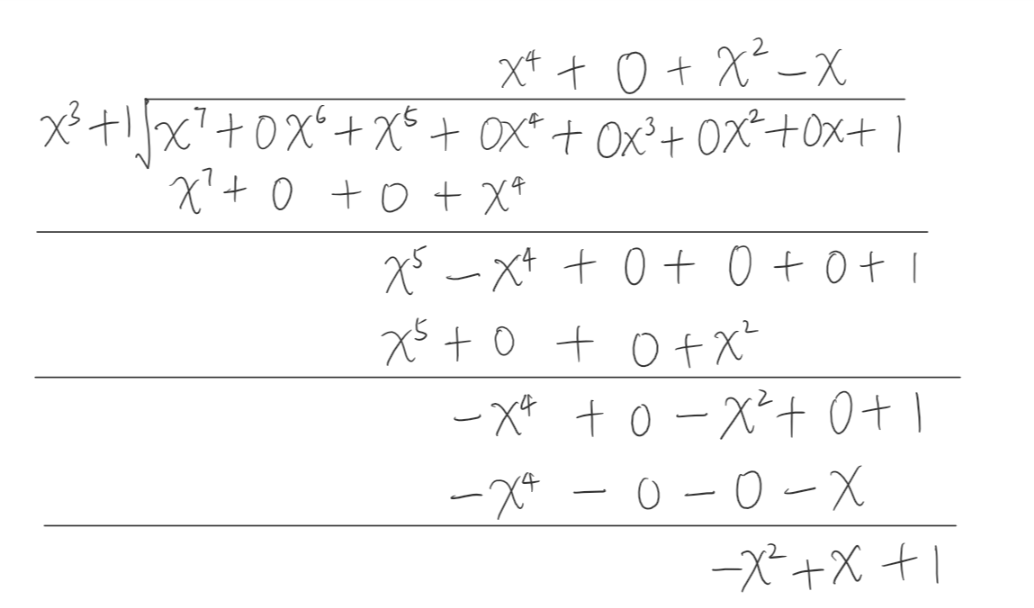
\includegraphics[width=0.6\linewidth]{q9.png}
\label{fig:q9}
\end{figure}\\
The remainder is $(-x^2 + x + 1)$
\end{homeworkProblem}
%----------------------------------------------------------------------------------------
%	PROBLEM 10
%----------------------------------------------------------------------------------------
\begin{homeworkProblem}
\noindent \textit{CRC}\\

a)\\
The message should be sent is 11100011100, where the last three bit '100' is remainder.\\
\begin{figure}[h!]
\centering
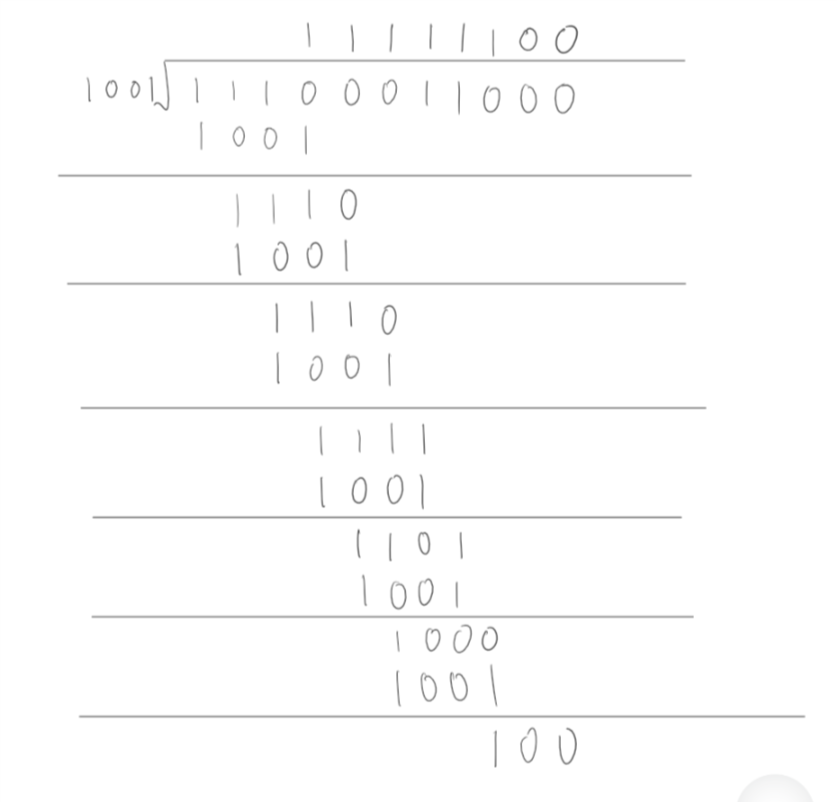
\includegraphics[width=0.6\linewidth]{q10a.png}
\label{fig:q10a}
\end{figure}\\
\clearpage

b)\\
Since we got a remainder when dividing the received message by the generator, it signals that there is an error during the transmission. There shouldn't be a remainder if the transmitted message is correct.\\
\begin{figure}[h!]
\centering
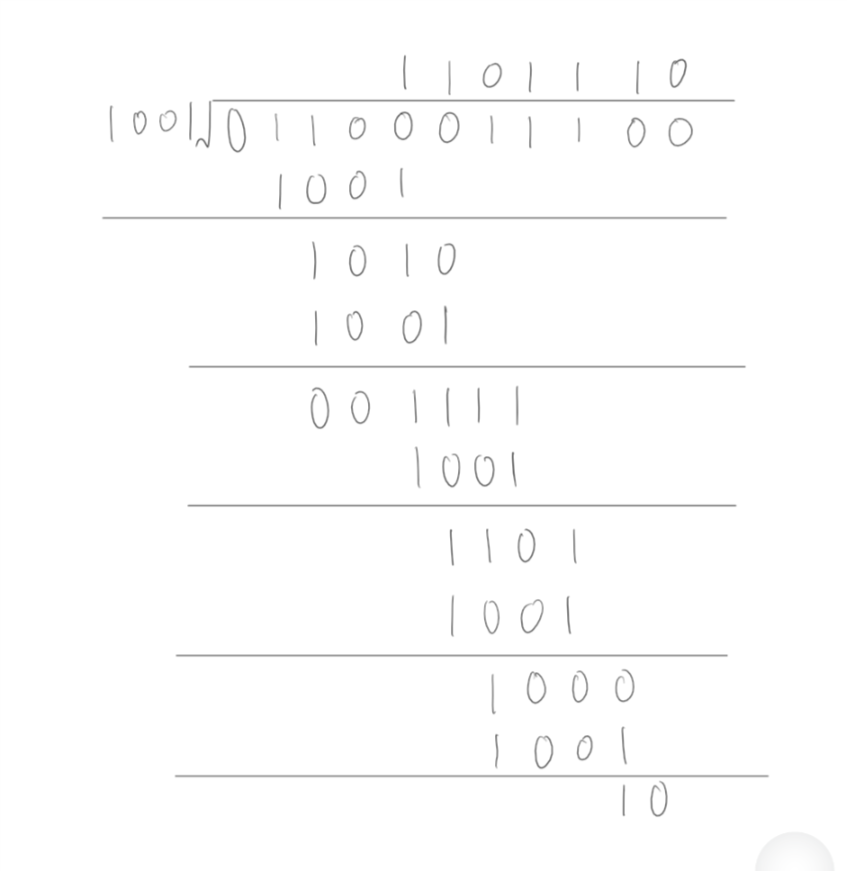
\includegraphics[width=0.6\linewidth]{q10b.png}
\label{fig:q10b}
\end{figure}\\

\end{homeworkProblem}
\clearpage
%----------------------------------------------------------------------------------------

\end{document}
